
\documentclass[ fontsize=11pt]{scrartcl} % A4 paper and 11pt font size

%%%%%%%%%%%%%%%%%%%%%%%%%%%%%%%%%%%%%%%%%%%%%%%%%%%%%%%%%%%%
%PICTURES
%%%%%%%%%%%%%%%%%%%%%%%%%%%%%%%%%%%%%%%%%%%%%%%%%%%%%%%%%%%%

\usepackage[]{graphicx} % for inserting figure, graphics,...
%\usepackage{subfigure} % conflict with subcaption
\usepackage{subcaption}

%%%%%%%%%%%%%%%%%%%%%%%%%%%%%%%%%%%%%%%%%%%%%%%%%%%%%%%%%%%%
%MARGINS & LAYOUT
%%%%%%%%%%%%%%%%%%%%%%%%%%%%%%%%%%%%%%%%%%%%%%%%%%%%%%%%%%%%
\usepackage{makeidx}

\usepackage{vmargin}
\setpapersize{A4}
\setmarginsrb{20mm}{5mm}{20mm}{15mm}
             {0mm}{7mm}{0mm}{10mm}
\setlength\parindent{0pt} % Removes all indentation from paragraphs - comment this line for an assignment with lots of text
\usepackage{array,makecell} %centering and manipulating cells in tables
%%%%%%%%%%%%%%%%%%%%%%%%%%%%%%%%%%%%%%%%%%%%%%%%%%%%%%%%%%%%
%LANGUAGE & FONT
%%%%%%%%%%%%%%%%%%%%%%%%%%%%%%%%%%%%%%%%%%%%%%%%%%%%%%%%%%%%

\usepackage[utf8]{inputenc} %& parole accentate (italiane!)

\usepackage{fourier} % Use the Adobe Utopia font for the document - comment this line to return to the LaTeX default
\usepackage[british]{babel} % English language/hyphenation

\usepackage{lipsum} % Used for inserting dummy 'Lorem ipsum' text into the template

\usepackage[T1]{fontenc} % Use 8-bit encoding that has 256 glyphs

\usepackage{fancyhdr} % Custom headers and footers
\pagestyle{fancyplain} % Makes all pages in the document conform to the custom headers and footers
\fancyhead{} % No page header - if you want one, create it in the same way as the footers below
\fancyfoot[L]{} % Empty left footer
\fancyfoot[C]{} % Empty center footer
\fancyfoot[R]{\thepage} % Page numbering for right footer
\renewcommand{\headrulewidth}{0pt} % Remove header underlines
\renewcommand{\footrulewidth}{0pt} % Remove footer underlines
\setlength{\headheight}{10.6pt} % Customize the height of the header

%%%%%%%%%%%%%%%%%%%%%%%%%%%%%%%%%%%%%%%%%%%%%%%%%%%%%%%%%%%%%%%
%MATH & PHYSICS
%%%%%%%%%%%%%%%%%%%%%%%%%%%%%%%%%%%%%%%%%%%%%%%%%%%%%%%%%%%%%%%
\usepackage{amsmath,amsfonts,amsthm} % Math packages
\usepackage{physics} %per scrivere veloce derivate parziali, ecc...
\usepackage{amssymb} %for gather and aligned type equation (multiline)
\usepackage{gensymb} %for degree symbol
\numberwithin{equation}{section} % Number equations within sections (i.e. 1.1, 1.2, 2.1, 2.2 instead of 1, 2, 3, 4)
\numberwithin{figure}{section} % Number figures within sections (i.e. 1.1, 1.2, 2.1, 2.2 instead of 1, 2, 3, 4)
\numberwithin{table}{section} % Number tables within sections (i.e. 1.1, 1.2, 2.1, 2.2 instead of 1, 2, 3, 4)
\usepackage{empheq} % for equation in box
\newcommand*\widefbox[1]{\fbox{\hspace{2em}#1\hspace{2em}}} %forboxes
\usepackage{enumitem} % for description (list of symbols chapter)
\usepackage{siunitx}

\newtheorem{myprop}{Property}
\newtheorem{myproof}{Proof}
\newtheorem{example}{Example}



%\usepackage{sectsty} % Allows customizing section commands
%\allsectionsfont{\centering \normalfont\scshape} % Make all sections centered, the default font and small caps


%%%%%%%%%%%%%%%%%%%%%%%%%%%%%%%%%%%%%%%%%%%%%%%%%%%%%%%%%%%%%%%%%%%%%%%%%%%%%%
%	TITLE SECTION
%%%%%%%%%%%%%%%%%%%%%%%%%%%%%%%%%%%%%%%%%%%%%%%%%%%%%%%%%%%%%%%%%%%%%%%%%%%%%%

\newcommand{\horrule}[1]{\rule{\linewidth}{#1}} % Create horizontal rule command with 1 argument of height

\title{	
\normalfont \normalsize 
\textsc{Istituto Nazionale di RIcerca Metrologica } \\ [10pt]
%\textsc{} \\ [10pt] % university, school and/or department name(s)
\horrule{0.7pt} \\[0.4cm] % Thin top horizontal rule
\huge Phase tracking and intensity fading due to polarization change in optical fibre link \\ % The assignment title
\horrule{3pt} \\[0.5cm] % Thick bottom horizontal rule
}

\author{Stefano Paracchino} % Your name

\date{October 2018} % Today's date or a custom date



%%%%%%%%%%%%%%%%%%%%%%%%%%%%%%%%%%%%%%%%%%%%%%%%%%%%%%%%%%%%%%%%%%%%%%%%%%%%%%%%
%%%%%%%%%%%%%%%%%%%%%%%%%%%%%%%%%%%%%%%%%%%%%%%%%%%%%%%%%%%%%%%%%%%%%%%%%%%%%%%%%
%%%%%%%%%%%%%%%%%%%%%%%%%%%%%%%%%%%%%%%%%%%%%%%%%%%%%%%%%%%%%%%%%%%%%%%%%%%%%%%%%%
\begin{document}

\maketitle
\tableofcontents 
\pagebreak

\section{Noise sensitivity of the algorithm}

Two kinds of random process  (at least)  must be taken into account in order to perform simulations with a good reliability:

\begin{itemize}
\item \textsl{intrinsic noise:} this is actually the metrological information we want to reveal. A clock stability as well as the optical link performance is measured in terms of noise power spectral density. In particular, considering that these measurements are based on the phase difference between two oscillators, we are interested in the phase noise power spectral density (PSD) $S_{\phi}(f)$ $\left(\frac{\text{rad}^2}{\text{Hz}}\right)$.
This quantity is usually modeled using a power-law function $S_{\phi}(f)=b_0 \, f^{0} + b_1 \, f^{-1}+ b_2 \, f^{-2}+ b_3 \, f^{-3}+...$ which corresponds, in the typical log-log plot, to a sum of lines with different slope.\\
Recalling that $S_{\phi}(f)$ is intended to be one-side PSD \footnote{The PSD of a real function is an even function. Furthermore the one-side PSD is what is displayed by a spectrum analyzer instrument.}, namely:
\begin{equation}
S(f)=\frac{2}{T}\left|\hat{X}(f)\right|^2
\end{equation}
where $T$ is the measurement time and $\left|\hat{X}(f)\right|^2$ is the Fourier Transform in the frequency domain $f$. \\
Moving to the digital domain, the one-side PSD becomes:
\begin{equation}
S(\mathtt{F})=\frac{2}{N\cdot f_s}\left|\hat{X}(F)\right|^2
\end{equation}
where $N$ is the number of samples and $f_s$ is the sampling frequency, while $F$ is the digital (discrete) frequency.\\
However for a preliminary analysis, a simpler model $S_{\phi}(f)=b_0 \, f^{0} + b_2 \, f^{-2}$ will be considered, whose terms are called respectively \textit{white noise}  and \textit{random walk (noise)}.  In this case, only two meaningful quantities must be known to fully describe the function: the $b_0$ factor for the white noise and the $b_2(1)^{-2}=b_2$ product i.e. the noise value at $f=1$ for the random walk term.

\item \textsl{detection noise:} this is due to the opto-electronic read-out system. In spite of the several phenomena involved for a complete noise description (shot noise, flickering,...) we choose a simplified model for a preliminary analysis as above. This takes  into account the only contribution of the white noise. In particular, the four channels are considered uncorrelated i.e. each one is characterized by a single white noise random process. 

\item \textsl{quantization noise:} this phenomenon arises from the ADC process. A correspondence between the time and frequency domains is quite complex to be derived, but the frequency spectrum can be assumed flat (i.e. quantization noise becomes white) for the whiteness condition \footnote{Eq (20.54) of http://oldweb.mit.bme.hu/books/quantization/spectrum.pdf}:
\begin{equation}
f_s<9.2 \frac{\sigma_x}{q}BW=9.2\frac{1}{\sqrt{12}}BW\approx 2.7BW
\end{equation}
The condition can be satisfied for an observed signal with a frequencies components which extend up to near the nyquist frequency.

\end{itemize}

In Digital Signal Process, random processes such as white noise and random walk are modeled with a sequence of data arising from random data generation. In the former case every value of the sequence is obtained with the formula $A_{\text{rw}} \cdot \mathcal{N}(0,1) $ where $\mathcal{N}(0,1) $ is a value randomly extracted from a Normal Distribution with zero mean and unitary variance while the values of a random walk sequence are $A_{\text{rn}} \cdot \mathcal{C}(\mathcal{N}(0,1) )$ where  $\mathcal{C}(\mathcal{N}(0,1) )$ is the cumulative sum of the white noise n-length sequence up to the considered n-th value.
The magnitudes of the amplitudes $A_{\text{wn}}$ and $A_{\text{rn}}$ are determined respectively by the chosen values for $b_0$ and $b_2$ as described in Tab.(\ref{pow-amp}):


\begin{table}[htb]
\centering
\begin{tabular}{cccll}
\cline{1-4}
\multicolumn{1}{|c|}{}                                                      & \multicolumn{1}{c|}{Amplitude} & \multicolumn{1}{c|}{PSD} & \multicolumn{1}{c|}{Applied to} &  \\ \cline{1-4}
\multicolumn{1}{|c|}{\begin{tabular}[c]{@{}c@{}}random\\ walk\end{tabular}} & \multicolumn{1}{c|}{$\sqrt{\frac{2 \pi^2 b_2}{f_s}}$ \SI{}{(\radian)}}          & \multicolumn{1}{c|}{$b_2(1)^{-2}=b_2$ \SI{}{(\radian\squared\per\hertz})}       & \multicolumn{1}{c|}{Simul. params} &  \\ \cline{1-4}
\multicolumn{1}{|c|}{\begin{tabular}[c]{@{}c@{}}white\\ noise\end{tabular}} & \multicolumn{1}{c|}{$\sqrt{\frac{b_0 f_s}{2}}$ \SI{}{(\radian)}}          & \multicolumn{1}{c|}{$b_0$ \SI{}{(\radian\squared\per\hertz})}      & \multicolumn{1}{c|}{Simul. electr. channels} &  \\ \cline{1-4}
\multicolumn{1}{|c|}{\begin{tabular}[c]{@{}c@{}}quant\\ noise\end{tabular}} & \multicolumn{1}{c|}{}          & \multicolumn{1}{c|}{}      & \multicolumn{1}{c|}{Simul. electr. channels} &  \\ \cline{1-4}
\multicolumn{1}{l}{}                                                        & \multicolumn{1}{l}{}           & \multicolumn{1}{l}{}       &  & 
\end{tabular}
\caption{Amplitude-PSD relation for random processes}
\label{pow-amp}
\end{table}
\pagebreak

The starting point for our noise sensitivity analysis is the choice of proper values for $b_0$ and $b_2$. Fig(\ref{psd_long}) a typical optical fiber link phase noise spectrum for a long distance distance link  ($\approx 100$ \SI{}{\kilo\meter}) while Fig(\ref{psd_short}) presents the phase noise spectrum obtained via the recovery algorithm, where the total length is limited for testing reason to just  few meters  and for a short distance (few meters).
\begin{figure}[hbtp]
\centering
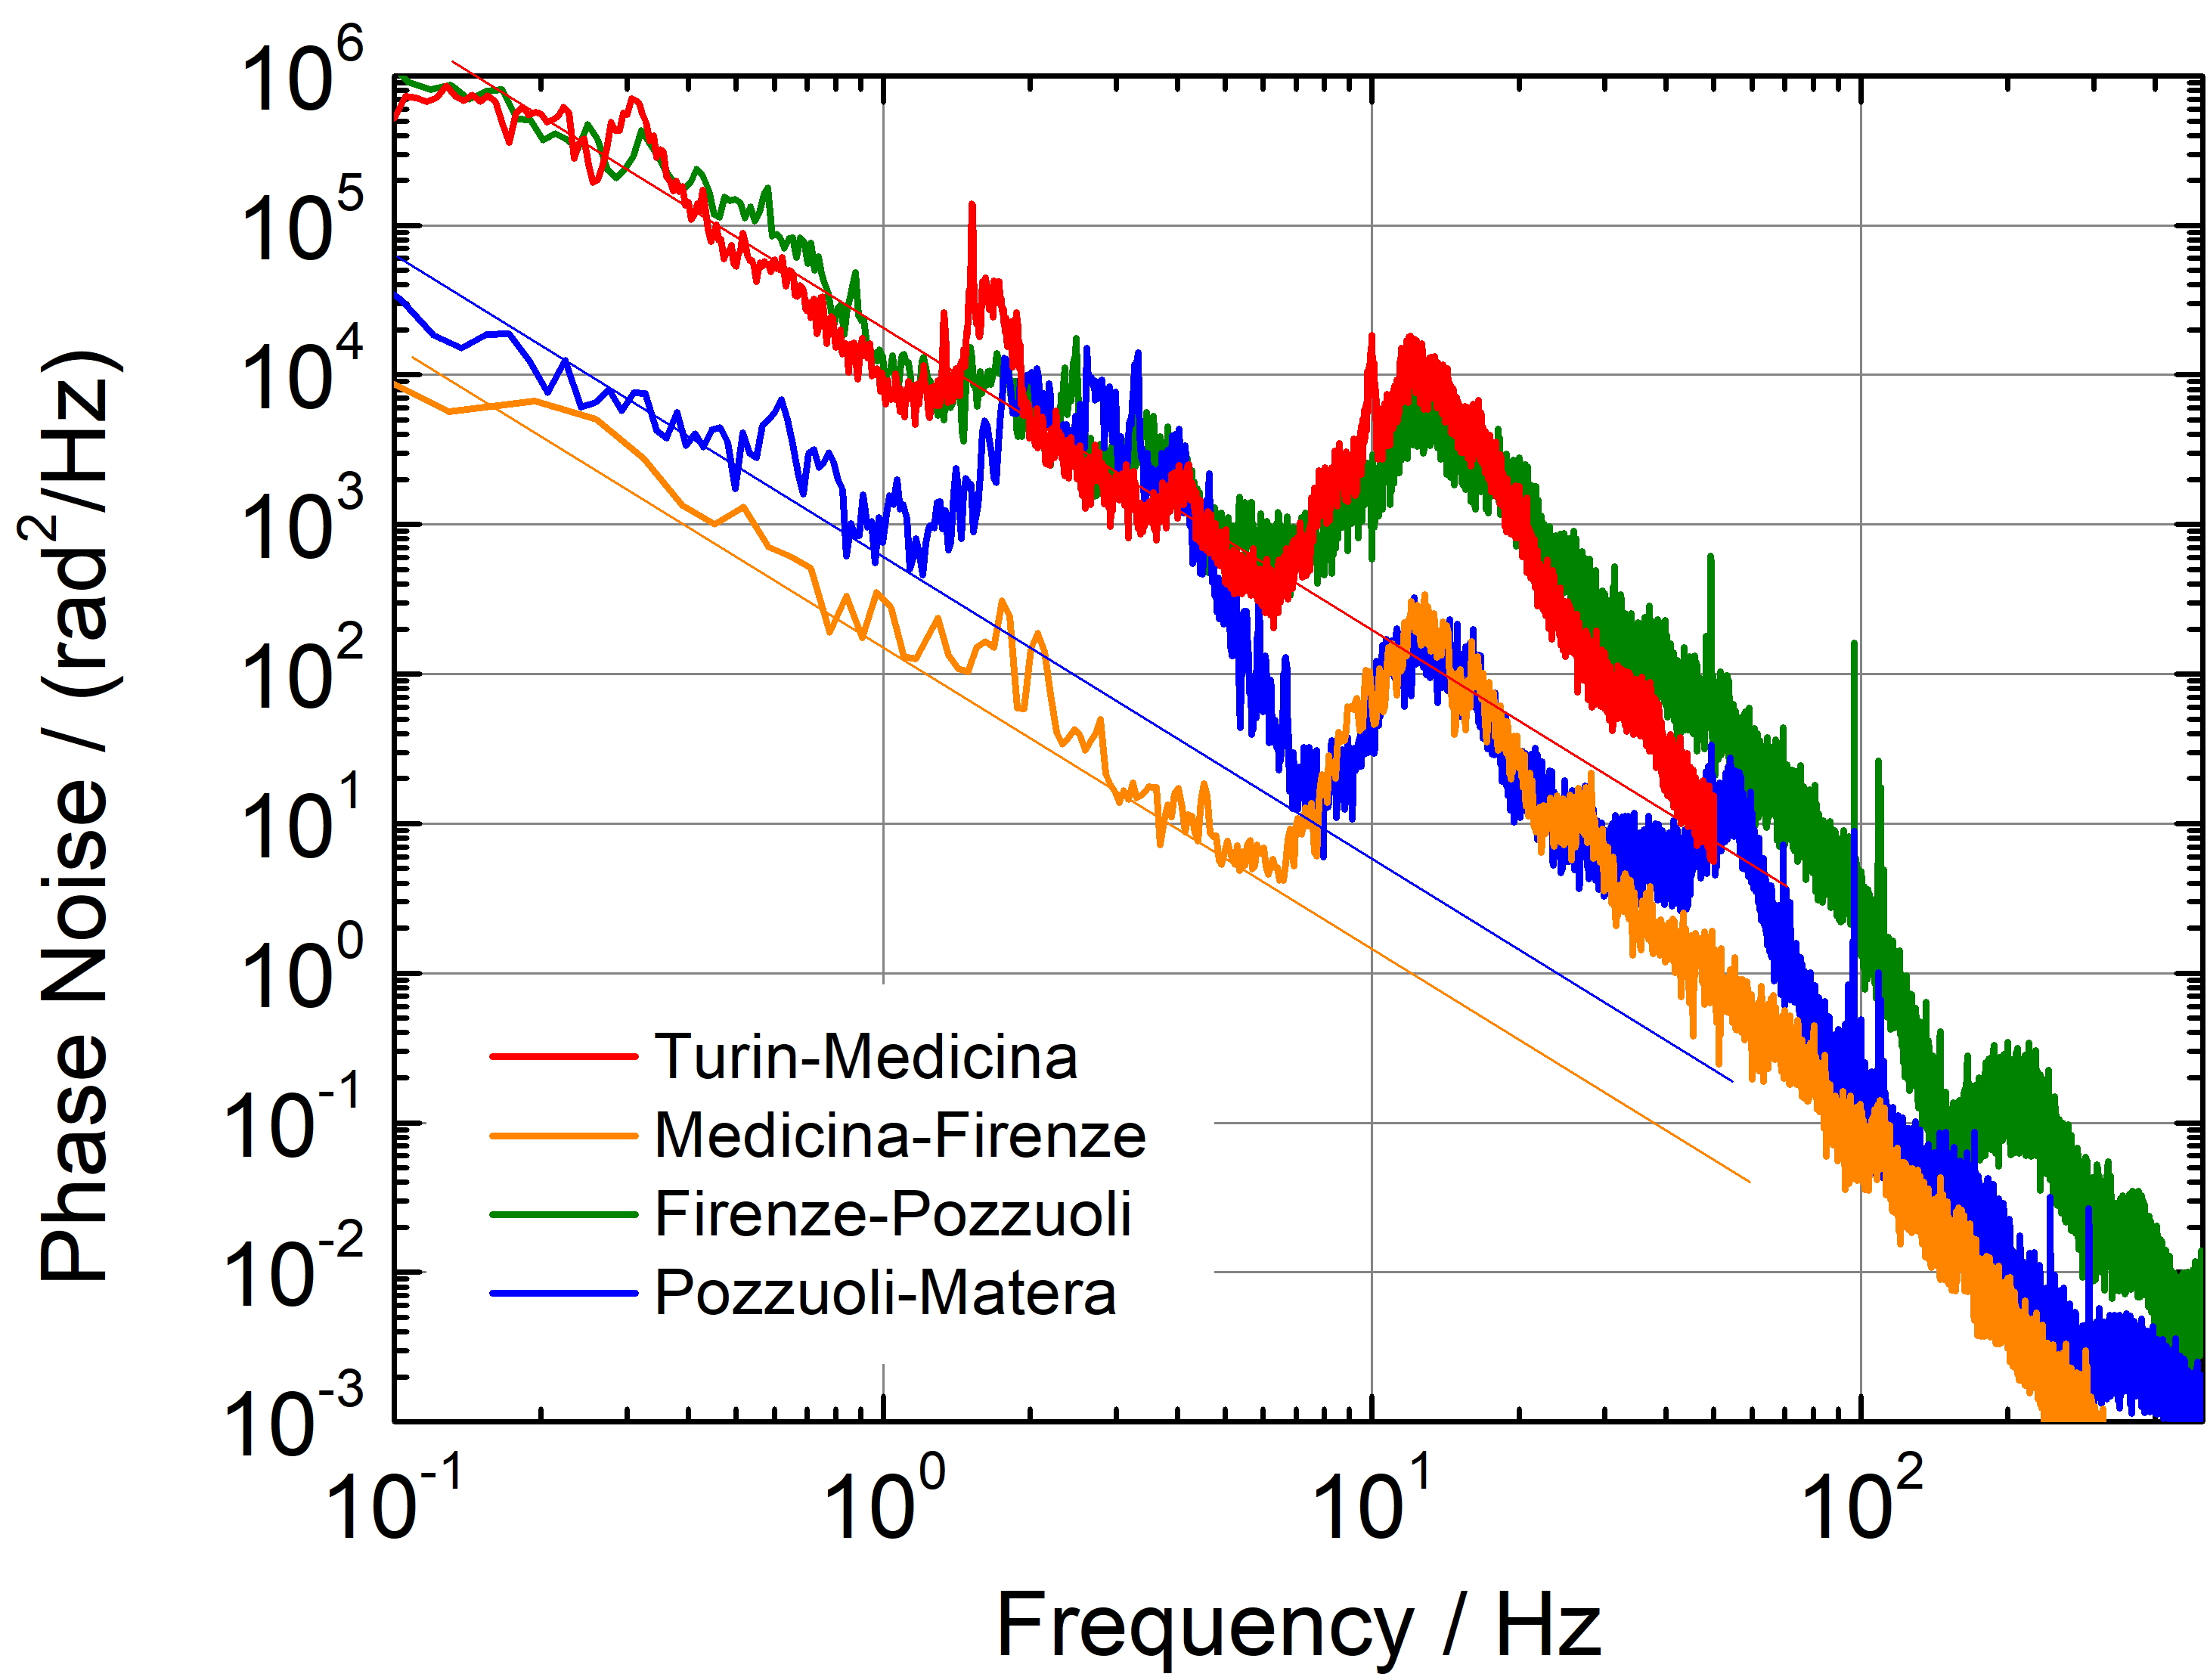
\includegraphics[scale=0.5]{immagini_noise/noise_long.png}
\caption{Phase PSD for a long distance link in a real frequency dissemination system}
\label{psd_long}
\end{figure}

\begin{figure}[hbtp]
\centering
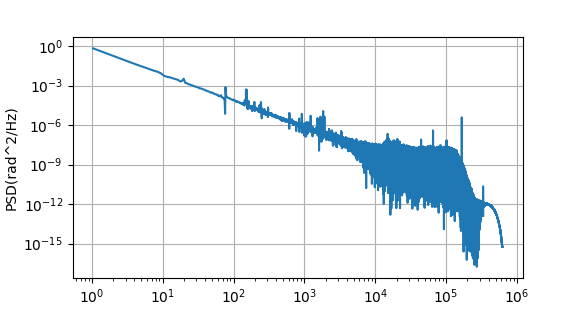
\includegraphics[scale=1]{immagini_noise/noise_short.png}
\caption{Phase PSD for a long short link in lab environment. (downsampling=2, lowfilter=100kHz)}
\label{psd_short}
\end{figure}



\end{document}
